\documentclass[landscape,24pt, a0paper,colspace=8mm,blockverticalspace=8mm]{tikzposter}

% Bibliography
%\usepackage[backend=bibtex,firstinits=true,sorting=none, doi=false,isbn=false,url=false]{biblatex}
%\bibliography{Mendeley.bib}
%\renewbibmacro{in:}{}
%\DeclareFieldFormat*{title}{#1} 

% Bibliography v2
%\usepackage[style=nature,maxnames=1,uniquelist=false]{biblatex}
\usepackage[backend=bibtex,giveninits=true,sorting=none, doi=false,isbn=false,url=false,maxnames=1,uniquelist=false]{biblatex}
\renewbibmacro{in:}{}
\DeclareFieldFormat*{title}{#1} 

% For shifting parts of the text left or right
\usepackage{changepage}

% For preventing hyphenation
\usepackage{hyphenat}
% e.g.    \nohyphens{longlineoftexthere}
    
% Some field suppression via options
\ExecuteBibliographyOptions{isbn=false,url=false,doi=false,eprint=false}

% One-paragraph bibliography environment
\defbibenvironment{bibliography}
  {\list
     {\printtext[labelnumberwidth]{%
        \printfield{labelprefix}%
        \printfield{labelnumber}}%
      \ifentrytype{article}{% Suppress remaining fields/names/lists here
        \clearfield{title}}{}}
     {\setlength{\leftmargin}{0pt}%
      \setlength{\topsep}{0pt}}%
      \renewcommand*{\makelabel}[1]{##1}}
  {\endlist}
  {\mkbibitem}

% \mkbibitem just prints item label and non-breakable space
\makeatletter
\newcommand{\mkbibitem}{\@itemlabel\addnbspace}
\makeatother

% Add breakable space between bibliography items
\renewcommand*{\finentrypunct}{\addperiod\space}

% et al. string upright (nature style applies \mkbibemph)
\renewbibmacro*{name:andothers}{%
  \ifboolexpr{
    test {\ifnumequal{\value{listcount}}{\value{liststop}}}
    and
    test \ifmorenames
  }
    {\ifnumgreater{\value{liststop}}{1}{\finalandcomma}{}%
     \andothersdelim
     \bibstring{andothers}}
    {}}

\addbibresource{Mendeley.bib}
 
 
%Remove 'references' title from bibliography
\usepackage{etoolbox}
\patchcmd{\thebibliography}{\section*{\refname}}{}{}{}

\usepackage{calculator}%For doing arithmetic?
\usepackage{verbatim}

\usepackage{amssymb, amsmath, mathrsfs, bm, mathtools}
\usepackage[makeroom]{cancel}

\newcommand{\Rm}{Rm}
\newcommand{\Da}{Da}
\newcommand{\Reynolds}{Re}
\newcommand{\Prandtl}{Pr}
\newcommand{\Ra}{Ra}

\newcommand{\St}{\mathscr{S}}
\newcommand{\ConcRatio}{\mathscr{C}}
\newcommand{\Le}{Le}


\newcommand*{\enthalpy}{\mathscr{H}}
\newcommand*{\RaT}{\ensuremath{Ra_T}}
\newcommand*{\RaTC}{\ensuremath{Ra_T^c}} %Critical rayleigh number
\newcommand*{\RaC}{\ensuremath{Ra_C}}
\newcommand*{\RaS}{\ensuremath{Ra_S}}
\newcommand*{\RmC}{\ensuremath{Rm_C}}
\newcommand*{\RmS}{\ensuremath{Rm_S}}
\newcommand*{\RmT}{\ensuremath{Rm_T}}
\newcommand*{\RmCrit}{\ensuremath{Rm_{crit}}}

\newcommand*{\Rmush}{\ensuremath{Rm}}
\newcommand*{\RaLiquid}{\ensuremath{Ra}}

\newcommand*{\RaCrit}{\ensuremath{Ra_c}}

\newcommand*{\Nu}{\ensuremath{Nu}}


\DeclareMathOperator\arctanh{arctanh}



% For displaying equations in tables
\usepackage{array}
%\def\tabularxcolumn#1{m{#1}} %ensure vertical centering
\newcolumntype{L}[1]{>{\raggedright\let\newline\\\arraybackslash\hspace{0pt}}m{#1}}
\newcolumntype{C}[1]{>{\centering\let\newline\\\arraybackslash\hspace{0pt}}m{#1}}
\newcolumntype{R}[1]{>{\raggedleft\let\newline\\\arraybackslash\hspace{0pt}}m{#1}}



\usepackage{authblk} %Formatting of author lists
\usepackage{enumitem} % For different itemize icons
\usepackage{graphicx,subcaption} % For subfigures
\usepackage{xcolor} %For colors in equations

%\definecolor{oxfordblue}{rgb}{0.0, 0.13, 0.28}
\definecolor{darkolivegreen}{rgb}{0.33, 0.42, 0.18}
\definecolor{darkmidnightblue}{rgb}{0.0, 0.2, 0.4}
\definecolor{darkpowderblue}{rgb}{0.0, 0.2, 0.6}
\definecolor{dodgerblue}{rgb}{0.12, 0.56, 1.0}
\definecolor{egyptianblue}{rgb}{0.06, 0.2, 0.65}
\definecolor{dukeblue}{rgb}{0.0, 0.0, 0.61}
\definecolor{falured}{rgb}{0.5, 0.09, 0.09}
\definecolor{royalfuchsia}{rgb}{0.79, 0.17, 0.57}

\definecolor{captiongray}{rgb}{0.15,0.15,0.15}
\definecolor{captionTitle}{rgb}{0, 0, 0}
\definecolor{dividingLines}{rgb}{0.7, 0.7, 0.7}
\definecolor{eqnLabelGray}{rgb}{0.3, 0.3, 0.3}
\definecolor{dividingLines}{rgb}{0.2, 0.2, 0.2}

\definecolor{keyPoint}{rgb}{0.0, 0.13, 0.28} % oxford blue

\newcommand{\keyPoint}[1]{\textcolor{darkpowderblue}{#1}}

\newcommand{\figureTitle}[1]{\color{captionTitle}{\textbf{#1}} }
\newcommand{\figureCaption}[1]{\color{captiongray}{#1} }

\newcommand{\highlightText}[1]{\textcolor{dukeblue}{\textbf{#1}} }

\newcommand{\varColor}[1]{\textcolor{dukeblue}{#1}}
\newcommand{\eqnColor}[1]{\textcolor{royalfuchsia}{#1}}
\newcommand{\paramColor}[1]{\textcolor{falured}{#1}}
\newcommand{\varLabel}[1]{\textcolor{eqnLabelGray}{\text{#1}}}

\newcommand{\eqnLabel}[1]{\textcolor{eqnLabelGray}{#1}}

\usepackage{pgfplots}
\usepgfplotslibrary{fillbetween}
\pgfplotsset{compat=1.13}

\usepackage{tikz}
\usetikzlibrary{calc,positioning,decorations.markings, backgrounds}

% Useful macro for finding out what the current font size is 
\makeatletter
\newcommand\thefontsize{{The current font size is: \f@size pt\par}}
\makeatother


\makeatletter

%24 pt for figure captions for AGU
\renewenvironment{tikzfigure}[1][]{
  \def \rememberparameter{#1}
  \vspace{10pt}
  \refstepcounter{figurecounter}
  \begin{center}
  }{
    \ifx\rememberparameter\@empty
    \else %nothing
    \\[24pt]
    {Fig.~\thefigurecounter: \rememberparameter}
    \fi
  \end{center}
}

% Title formatting
\def\TP@titlegraphictotitledistance{-5.0cm} % Without this, authors are below icons

\renewcommand\AB@affilsepx{, \protect\Affilfont}

\settitle{ \centering \vbox{

\centering
\vspace{-2.0cm}
\color{titlefgcolor} {\bfseries \Huge \sc \@title \par}
\vspace*{0.5cm} % Distance from bottom of title to top of graphics
% For title graphics. Uncomment next line to remove
\@titlegraphic \\ [\TP@titlegraphictotitledistance] 
{\LARGE \@author \par} \vspace*{0.8em} {\Large \@institute}
\vspace*{-5em}
}
}

\def\maketitle{\AB@maketitle} % prevent shifing content block to middle of page

\makeatother

%Define my block style
\defineblockstyle{MyBlock}{% define a custom style for a block
    titlewidthscale=1.0, bodywidthscale=1, titleleft,
    titleoffsetx=0pt, titleoffsety=0pt, bodyoffsetx=0pt, bodyoffsety=26mm,
    bodyverticalshift=16mm, roundedcorners=22, linewidth=5pt,
    titleinnersep=7mm, bodyinnersep=8mm
}{
    \draw[rounded corners=\blockroundedcorners, inner sep=\blockbodyinnersep,
          line width=\blocklinewidth, color=blocktitlefgcolor,
          top color=titlebgcolor, bottom color=titlebgcolor,
          fill=blockbodybgcolor
          ]
      (blockbody.south west) rectangle (blockbody.north east); %
    %\ifBlockHasTitle%
    %    \draw[rounded corners=\blockroundedcorners, inner sep=\blocktitleinnersep,
    %      top color=titlebgcolor!90, bottom color=titlebgcolor!20!white,
    %      line width=\blocklinewidth, color=black, %fill=blocktitlebgcolor
    %      ]
    %  (blocktitle.south west) rectangle (blocktitle.north east); %
    %\fi
}
\newcommand\myblock[3][MyBlock]{\useblockstyle{#1}\block{#2}{#3}\useblockstyle{Basic}}



% Theme details
\usetheme{Default} % See Section 5
\usebackgroundstyle{Empty}
\usetitlestyle[width=0.98\textwidth]{Default} 
\useblockstyle{MyBlock}

\definecolor{oxfordblue}{rgb}{0.0, 0.13, 0.28}

\definecolorstyle{sampleColorStyle} 
{
\definecolor{colorOne}{named}{blue}
\definecolor{colorTwo}{named}{yellow}
\definecolor{colorThree}{named}{orange} 
}{
% Background Colors
\colorlet{backgroundcolor}{white}
\colorlet{framecolor}{white}
% Title Colors
\colorlet{titlefgcolor}{oxfordblue}
\colorlet{titlebgcolor}{white} % white
% Block Colors
\colorlet{blocktitlebgcolor}{white} %oxfordblue
\colorlet{blocktitlefgcolor}{oxfordblue}
\colorlet{blockbodybgcolor}{oxfordblue} % white
\colorlet{blockbodyfgcolor}{black}
% Innerblock Colors
\colorlet{innerblocktitlebgcolor}{white}
\colorlet{innerblocktitlefgcolor}{black}
\colorlet{innerblockbodybgcolor}{colorThree!30!white}
\colorlet{innerblockbodyfgcolor}{black}
% Note colors
\colorlet{notefgcolor}{black}
\colorlet{notebgcolor}{colorTwo!50!white}
\colorlet{noteframecolor}{colorTwo}
}

\usecolorstyle[]{sampleColorStyle}

%\definecolor{MyYellow}{RGB}{175 141 38}

\usepackage{mdframed}
\newmdenv[topline=false,
leftline=false,
bottomline=false,
linewidth=1.5mm,
linecolor=oxfordblue,
skipabove=-20em,
innertopmargin=0em]{leftbot}


\usepackage{tcolorbox}
\tcbset{arc=20pt,
        leftright skip=-0.92em,
        after skip=-0.92em,
        boxrule=1.6mm}

%Title text and graphics
\title{\parbox{\linewidth}{\centering Convection, phase change, and solute transport in mushy sea ice}} %with Adaptive Mesh Refinement
\titlegraphic{ \includegraphics[height=4cm]{figures/EGU2019Website.eps} %TODO: update QR code

\includegraphics[height=4cm]{figures/Oxford.eps}

\includegraphics[height=4cm]{figures/Berkeley_Lab_Logo_Small.eps} 
 \hfill 
  
\includegraphics[height=4cm]{figures/nerc-logo.eps}  
     
\includegraphics[height=4cm]{figures/roysoclogo.jpg} 
}
%For now title graphic:
%\titlegraphic{}

% Authors
\author[1]{James Parkinson (james.parkinson@physics.ox.ac.uk)}
\author[1]{Andrew Wells}
\author[2]{Dan Martin}
\author[1]{Richard Katz}

\affil[1]{University of Oxford}
\affil[2]{Lawrence Berkeley National Laboratory}



\tikzposterlatexaffectionproofoff % get rid of watermark in bottom right corner


 \tikzset{->-/.style={decoration={
  markings,
  mark=at position .5 with {\arrow[scale=2]{latex}}},postaction={decorate}}}


\begin{document}

\maketitle

\begin{columns} 

\column{0.22}

\block{Motivation}{
\begin{itemize}[leftmargin=0.4cm]
    \item Sea ice is a mushy layer of ice crystals and brine.
    \item Dense brine drains during ice formation, whilst some brine is trapped within sea ice
    \item Observations (Fig. 1) and 1-D simulations suggest that warming sea ice may release some of this brine
    \item \textbf{Our goal: investigate this mechanism} using \mbox{2-D} numerical simulations
\end{itemize}
\vspace{-1em}
\noindent


\begin{adjustwidth}{-1em}{0em}

\begin{tikzfigure}
\label{fig:widellObs}
\begin{tikzpicture}

\node[anchor=north west] (fig2) at (0,0) {\includegraphics[width=0.98\linewidth, trim={0.0cm, 0.0cm, 0.0cm, 0.0cm}, clip]{figures/widdellFig1TaToFsTimeCropped.png} };

\end{tikzpicture}
\end{tikzfigure}
\end{adjustwidth}
\figureTitle{Fig. 1:} \figureCaption{\cite{Widell2006} observed intense salt fluxes $F_s$ below sea ice coincident with changes to the temperature in the atmosphere ($T_a$) and ocean ($T$).}




}


\block{What is a mushy layer?}
{
\vspace{-0cm}

\begin{tikzfigure}
\label{fig:phaseDiagram}
\begin{tikzpicture}

\node[anchor=north west] (fig2) at (0,0) {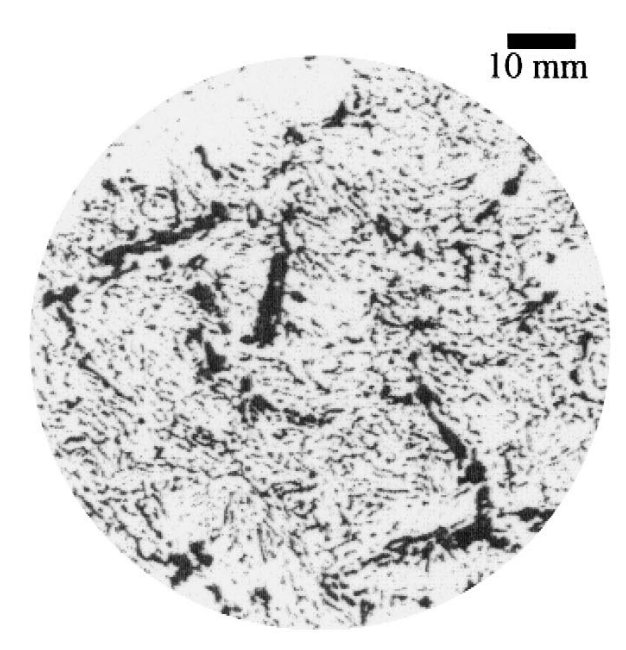
\includegraphics[width=0.4\linewidth, trim={0.0cm, 0.0cm, 0.0cm, 0.0cm}, clip]{figures/Eicken2000Edited.jpg} };

\node[anchor=north west] (phaseDiagram) at ([xshift=1.0cm]fig2.north east) {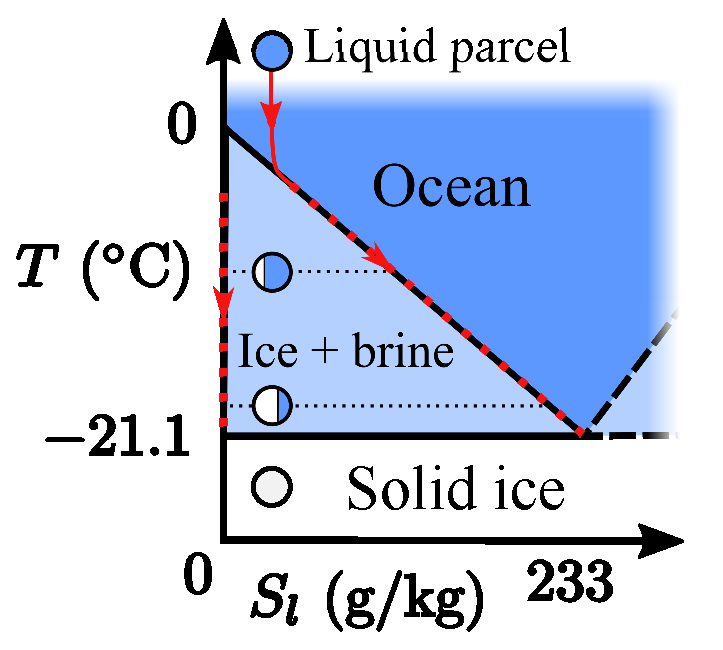
\includegraphics[width=0.47\linewidth, trim={0.0cm, 0.0cm, 0.0cm, 0.0cm}, clip]{figures/phaseDiagramVFinal.eps} };

\node[anchor=north west] (fig2label) at (fig2.north west) {(a)};

\node[anchor=north west] (fig1label) at ([yshift=0.0cm]phaseDiagram.north west) {(b)};

\end{tikzpicture}
\end{tikzfigure}
\figureTitle{Fig. 2:} \figureCaption{(a) Sea ice is a porous mixture of solid ice crystals (white) and liquid brine (dark) \cite{Eicken2000}. \\
(b) Trajectory ($\textcolor{red}{\rightarrow}$) of a solidifying salt water parcel through the phase diagram. As the temperature $T$ decreases, more ice forms and the residual brine salinity $S_l$ increases making the fluid denser, which can drive convection. Using a linear approximation for the liquidus curve, the freezing point is $T_f(S_l) = -0.1 S_l$. }
%Below the eutectic ($T_e, S_e$) = (-21.1$^\circ$, 233) the system is entirely solid.} %making the fluid denser which can lead to convection
%the resulting dense fluid can drive convection
%Eicken et. al. (2000).
}
\block{Numerical Method}
{
\vspace{0.5em}
Solve (1)-(4) using Chombo finite volume toolkit:
\begin{itemize}
    \item Momentum and mass: projection method \cite{Martin2008}.
    \item Energy and solute:
   
 
    {
    \raggedright % left align - prevent splitting words over multiple lines as we have space
   \begin{itemize}    
   \item Advective terms: explicit, 2\textsuperscript{nd} order unsplit Godunov method. %\cite{Colella1990}, 
   \item Nonlinear diffusive terms: semi implicit, geometric multigrid. %\cite{Martin1996}
   \item Timestepping: Backward Euler. %\cite{Twizell1996} 
   \end{itemize}
   }
  % }
\end{itemize}
\vspace{-1ex}
}






\column{0.78}


\block[bodyoffsety=0em]{}{

\vspace{-2.6em}

%%%%%%%%%%%%%%%%%%%%%%%%%%%%%%%%
% Start experiment introduction
% sharp corners = uphill
%\begin{tcolorbox}[boxsep=5mm, % internal spacing
%width=0.5\linewidth+0.5em,  nobeforeafter, sharp corners, rounded corners=northwest,
%        colback=blue!5,  box align=top, 
%        colframe=oxfordblue, 
%        before skip=0.0em,
%        left skip=-0.9em,
%        boxrule=1.5mm, extrude top by=0.7em, arc=6mm,
%        height=8em]
        \begin{tcolorbox}[boxsep=5mm, % internal spacing
width=0.5\linewidth+0.8em,  nobeforeafter, 
sharp corners, 
%rounded corners=north,
 rounded corners=northwest,
        colback=blue!5,  box align=top, 
        colframe=oxfordblue, 
        before skip=0.0em,
        left skip=-0.9em,
        boxrule=1.5mm, extrude top by=0.7em, arc=6mm,
        height=9em]
\vspace{-1.0em}
%\begin{minipage}[t]{0.5\linewidth}
{\LARGE \textbf{The experiment:}} \\
We consider 2-D simulations in a Hele-Shaw cell of width $0.5$m, height $1$m, and plate separation $d$. Water of initial salinity $S_0=30\,\mathrm{g}/ \mathrm{kg}$ and temperature $T_f(S_o) + 0.2^\circ$C is initially frozen from above by applying a fixed atmospheric temperature $T_a = -10^\circ$C. We assume $K_0=10^{-9}\,\mathrm{m}^2$, and initially set $d=0.5$mm to restrict thermal convection in the underlying liquid during growth. After $\sim0.5$m of ice growth, we increase $d$ to $2$mm and spin up simulations for 2 days before considering different warming scenarios.
%\end{minipage} \hfill \textcolor{dividingLines}{\vline  width 1pt} \hfill
%\begin{minipage}[t]{0.16\linewidth}
%\vspace{-2.0em}
%\begin{tikzfigure}
%\begin{tikzpicture}
%\node[anchor=north west] (2d) at (0,0) {\includegraphics[ trim={0.0cm, 0.0cm, 0.0cm, 0.0cm}, clip]{figures/prePerturbationSmall.png}};
%\end{tikzpicture}
%\end{tikzfigure}
%\end{minipage} \hfill
%\begin{minipage}[t]{0.32\linewidth}
%\vspace{0.0em}

%\end{minipage} 

\end{tcolorbox} % \hfill
%% Summary
\begin{tcolorbox}[boxsep=5mm, width=0.5\linewidth+0.8em,  nobeforeafter, sharp corners, rounded corners=northeast,
        colback=red!5, box align=top, 
        colframe=red!60!black,  boxrule=1.5mm, extrude top by=0.7em, arc=6mm,
        height=9em, left skip=0.5em]

\vspace{-1.0em}
\LARGE \textbf{Summary}
\large 
\begin{itemize}
\item \textbf{We observe significant desalination events from warming sea ice in a 2-D model, with similar magnitude and timing to field observations.}
\item \textbf{Following basal melting, desalination can be caused by fresh melt water rising through brine channels.} 
%\item \textbf{...}
\end{itemize}
\end{tcolorbox}
% End summary
%%%%%%%%%%%%%%%%%%%%%%%%%%%%%%%%


% Nudge content up a bit
\vspace{-0.1em}


\begin{minipage}[t]{0.32\linewidth}
\vspace{1.0em}
{\LARGE \textcolor{oxfordblue}{\hspace{0.0em}\textbf{Full depth desalination}} }
\vspace{1em} \\
\noindent \figureTitle{Fig. 7 ($\rightarrow$):} Porosity $\chi$ in the ice, salinity $S_l$ in the underlying  liquid, and streamfunction (solid black logarithmically spaced contours: CW, dashed: ACW) during basal melting. Remnant brine channels are visible throughout the ice during initial growth. Subsequently the ocean temperature is increased to $T_o=T_f(S_o) + 1.5^{\circ}\mathrm{C}$ and a layer of buoyant water forms due to basal melting, whilst internal melting within the ice gradually increases the porosity. After 32 days a period of strong convection is initiated throughout the ice. Melt water rises through previously active brine channels and sinks through the rest of the ice.

%Our domain is horizontally periodic, with an open bottom boundary and an impermeable, isothermal, top boundary.
\end{minipage} \hfill
\begin{minipage}[t]{0.7\linewidth}
\begin{tikzfigure}
\begin{tikzpicture}
\node[anchor=north west] (diags) at (0,0) {\includegraphics[ trim={1.0cm, 0.0cm, 0.0cm, 0.0cm}, clip]{figures/desalinationEvent-small.png} };
\end{tikzpicture}
\end{tikzfigure}
\end{minipage}

\vspace{-2pt}
\begin{minipage}{\linewidth + 1.5em}
\hspace{-0.75em}\textcolor{dividingLines}{\rule{\linewidth}{3pt}}
\end{minipage}
\vspace{-3.0em} 

 
%%%%%%%%%%%%%%%%%%%%%%%%%%%%%%%%
% Case 1
\begin{tcolorbox}[width=0.5\linewidth+0.8em, nobeforeafter, box align=top, 
bottomrule=0pt, 
colframe=white, colback=white,  boxrule=0mm,
left skip=-1.0em,  left=0.0em, top=0.5em, right=0.5em,
bottom=0.4em,
 standard jigsaw, opacityback=0]

{\LARGE \textcolor{oxfordblue}{\hspace{1em}\textbf{Case 1: Atmospheric warming}}} 
\vspace{-1.5em}

\begin{tikzfigure}
\begin{tikzpicture}

\node[anchor=north west] (diags) at (0,0) {\includegraphics[trim={0.0cm, 0.0cm, 0.0cm, 0.0cm}, clip]{figures/SurfaceWarmingDiagnosticsNew.pdf} };

\node[anchor=north west] (timeseries2) at ([xshift=-1em,yshift=0]diags.north east) {\includegraphics[ trim={0.0cm, 0.0cm, 0.0cm, 0.0cm}, clip]{figures/SurfaceWarming-3TimeSeries-small.jpg}};

\node[anchor=north](b) at (timeseries2.north) {$T_a = -3^\circ$C};

\node[anchor=north](desalination) at ([xshift=-9.0em, yshift=5.0em]diags.south east) {\normalsize Desalination events};

\draw[->, line width=1mm](desalination.west) -- ([xshift=5.9em,yshift=3.7em]diags.south west);
\draw[->, line width=1mm](desalination.west) -- ([xshift=7.1em,yshift=5.6em]diags.south west);
\draw[->, line width=1mm](desalination.west) -- ([xshift=10.0em,yshift=5.4em]diags.south west);
\end{tikzpicture}
\end{tikzfigure}

\vspace{-2.0em}

\begin{minipage}[t]{1.0em} \end{minipage} \hfill % add some padding
\begin{minipage}[t]{0.39\linewidth}
\figureTitle{Fig. 3 ($\uparrow$):} Vertical fluxes of heat $F_h$ and salt $F_s$ at $z=0.3$m in response to increased atmospheric temperature (see legend).  %Intense desalination events can be seen for $T_a=-3^\circ$C (at $t=$2 days) and $-2^\circ$C (at $t=4$ and $8$ days). After $\sim 15$ days the warming ice stops rejecting significant quantities of salt. 
\keyPoint{Short intense desalination events occur after warming.} After $\sim 15$ days the warming ice stops rejecting significant quantities of salt. 
\end{minipage} \hfill
\begin{minipage}[t]{0.48\linewidth}
\figureTitle{Fig. 4 ($\uparrow$):} Vertical profiles for $T_a = -3^\circ$C. Top panel: minimum vertical velocity, middle panel: change in horizontally-averaged porosity, bottom panel: change in horizontally-averaged bulk salinity. The sea ice interface is indicated by a white line (top panel) or black line (lower panels). \keyPoint{Atmospheric warming increases the ice porosity, which allows salt to drain through the entire depth of ice.}
\end{minipage} 
%\hfill
%\begin{minipage}[t]{0.0em} \end{minipage}


\end{tcolorbox} \hfill \textcolor{dividingLines}{\vline  width 3pt} \hfill
%%%%%%%%%%%%%%%%%%%%%%%%%%%%%%%%
% Case 2
\begin{tcolorbox}[width=0.5\linewidth+0.5em, nobeforeafter, box align=top, 
top=0.5em,  left=-0.15em, right=0.5em,
boxrule=0mm, colback=white, colframe=white,  standard jigsaw, opacityback=0]


{\LARGE \textcolor{oxfordblue}{\hspace{1em}\textbf{Case 2: Basal warming}} }
\vspace{-1.5em}

%\begin{minipage}[t]{0.48\linewidth}
\begin{tikzfigure}
\begin{tikzpicture}

\node[anchor=north west] (diags) at (0,0) {\includegraphics[ trim={0.0cm, 0.0cm, 0.0cm, 0.0cm}, clip]{figures/BasalWarmingDiagnosticsNew.pdf} };

\node[anchor=north west] (timeseries2) at ([xshift=-1.5em,yshift=0]diags.north east) {\includegraphics[ trim={0.2cm, 0.0cm, 0.5cm, 0.0cm}, clip]{figures/BasalWarming-1p5TimeSeries-small.jpg}};

\node[anchor=north](b) at (timeseries2.north) {$T_o = T_f(S_o) + 1.5^\circ$C};

\node[anchor=north](desalination) at ([xshift=10.0em, yshift=5.0em]diags.south west) {\normalsize Desalination events};

\draw[->, line width=1mm]([xshift=-2.0em]desalination.north) -- ([xshift=7.3em,yshift=6.6em]diags.south west);
\draw[->, line width=1mm](desalination.east) -- ([xshift=16.5em,yshift=5.5em]diags.south west);
\draw[->, line width=1mm](desalination.east) -- ([xshift=19.0em,yshift=3.7em]diags.south west);

\node[anchor=north](desalination2) at ([xshift=8.0em, yshift=5.0em]timeseries2.south west) {\normalsize \textcolor{red}{Desalination event}};
% \draw ([xshift=-8.5em,yshift=1em]timeseries2.east) ellipse (1cm and 8cm);
\draw [rounded corners=0.5cm, red, line width=1mm] ([xshift=2.5em,yshift=4em]timeseries2.south) rectangle ++(1.8,15.5);
\draw[->, line width=1mm, red](desalination2.east) -- ([xshift=2em,yshift=4.5em]timeseries2.south);



\end{tikzpicture}
\end{tikzfigure}
\vspace{-2.0em}
\begin{minipage}[t]{1.0em} \end{minipage} \hfill % add some padding
\begin{minipage}[t]{0.39\linewidth}
\figureTitle{Fig. 5 ($\uparrow$):}  Vertical heat $F_h$ and salt $F_s$ fluxes as in Fig. 4 but for simulations with an increased oceanic temperature $T_o$. Salt fluxes are typically positive due to the downward transport of fresh melt water. However, for $T_o>T_f(S_o) + 0.5^\circ$C we observe short intense bursts of negative salt fluxes.
\end{minipage}\hfill
\begin{minipage}[t]{0.47\linewidth}
\figureTitle{Fig. 6 ($\uparrow$):}  Vertical profiles as in Fig. 5, but for oceanic warming with $T_o=T_f(S_o) + 1.5^\circ$C.  An increase in porosity permits stronger convection through a deeper layer at the base of the ice. However \keyPoint{a convectively stable layer of buoyant melt water forms below the ice, preventing rejected salt from mixing with the underlying ocean except in the case of intense desalination events.}
\end{minipage}


\end{tcolorbox}




%\vspace{-2em}

%%%%%%%%%%%%%%%%
% Summary
%\begin{tcolorbox}[boxsep=5mm, width=\linewidth+1.85em,  nobeforeafter, 
%sharp corners, rounded corners=south,
  %      colback=red!5, box align=top, 
     %   colframe=red!60!black,  boxrule=1.6mm, extrude bottom  by=0.1em, arc=6mm,
       % before skip=-1em,
       % height=3em]

%\vspace{0.1em}
%\LARGE \textbf{Summary:} {\Large We observe significant desalination events from warming sea ice in a 2-D model, with similar magnitude and timing to field observations.}
%\end{tcolorbox}

\vspace{-0.9em} } 
%%%%%%%%%%%%%%%%%%%%%%%%%%%%%%%%
% end big main block
%%%%%%%%%%%%%%%%%%%%%%%%%%%%%%%%

\begin{subcolumns}  
\subcolumn{0.75} 



\block{Governing Equations for Flow in Porous Mushy Sea Ice}
{

\begin{minipage}[t]{0.49\linewidth}
Continuous equations for conservation of momentum (1), mass (2), salt~\eqref{eq:salt-cons} and energy~\eqref{eq:energy-cons} are found by averaging over lengths greater than the pore scale of sea ice \cite{Worster1991,LeBars2006}. In a narrow Hele-Shaw cell, the momentum equation is well approximated by Darcy's law everywhere. 
\vspace{0.2em}
\begin{align}

%\mathbf{U} = \frac{K(\chi)}{\eta} \left( \rho_l \mathbf{g} - \nabla p \right), \quad \quad   \nabla \cdot \mathbf{U} &= 0,   \tag*{(1, 2)}\label{eq:mom-mass} \\
%    \frac{\partial S}{\partial t} + \mathbf{U} \cdot \nabla S_l &= \nabla \cdot \chi D_l \nabla S_l, \label{eq:salt-cons} \tag*{(3)} \\
%    \frac{\partial H}{\partial t} + \rho_0 \, c_{p,l} \, \mathbf{U} \cdot \nabla  T &= \nabla \cdot \left[ k_l \chi + (1-\chi) k_s \right] \nabla T . \label{eq:energy-cons} \tag*{(4)}

%\rho_0  \frac{\partial \mathbf{U}}{\partial \tau} + \rho_0 \mathbf{U} \cdot \nabla \left( \frac{\mathbf{U}}{\chi} \right) &= - \chi \nabla p + \eta \nabla^2 \mathbf{U} + \chi \rho_l \mathbf{g} - \frac{\eta \chi}{K(\chi)} \mathbf{U},
     \mathbf{U} = -\frac{K(\chi)}{\eta} \left(\nabla p - \rho_l \mathbf{g} \right), & \quad \quad   \nabla \cdot \mathbf{U} = 0, \tag{1, 2}  \\
    \frac{\partial S}{\partial t} + \mathbf{U} \cdot \nabla S_l &= \nabla \cdot \chi D_l \nabla S_l, \label{eq:salt-cons} \tag{3} \\
    \frac{\partial H}{\partial t} + \rho_0 \, c_{p,l} \, \mathbf{U} \cdot \nabla  T &= \nabla \cdot \left[ k_l \chi + (1-\chi) k_s \right] \nabla T . \label{eq:energy-cons} \tag{4}

\end{align} 
\end{minipage}
\hfill
\begin{minipage}[t][][b]{0.48\linewidth}
\vspace{-1.0\baselineskip}
\begin{align*}
&\varColor{\mathbf{U}}\; \text{(Darcy velocity)}, \quad \varColor{\chi} \; \text{(porosity)}, \quad \varColor{p} \; \text{(pressure)}, \quad \varColor{T} \; \text{(temperature)},\\
&\varColor{S_l} \; \text{(liquid salinity)}, \quad \varColor{S = \chi S_l} \; \text{(bulk salinity)},  \\
&\eqnColor{H = \rho_0 \left\{ L \chi + \left[\chi c_{p,l} + (1-\chi) c_{p,s}\right] T \right\}} \; \text{(enthalpy)}, \\
&\eqnColor{\rho_l = \rho_0 \left[1 - \alpha T + \beta S_l \right]} \; \text{(liquid density)}, \\
&\eqnColor{K(\chi)^{-1} = \left(d^2/12\right)^{-1} + \left[K_0 \chi^3 / (1-\chi)^2 \right]^{-1}} \; \text{(permeability)}, \\
&\paramColor{\eta} \; \text{(viscosity)}; \paramColor{D_l} \; \text{(salt diffusivity)}; \paramColor{\alpha}, \paramColor{\beta} \; \text{(thermal/haline expansion)}; \\
&\paramColor{c_{p,l}}, \paramColor{c_{p,s}} \; \text{(liquid/solid specific heat)}; \paramColor{k_l}, \paramColor{k_s} \; \text{(liquid/solid heat conductivity)}; \\
&\paramColor{d} \; \text{(Hele-Shaw cell thickness)}; \paramColor{K_0} \; \text{(Reference permeability)}.
\end{align*}
\end{minipage}

}
 

\subcolumn{0.25}
 
 \block{Future Work}
{

\begin{itemize}
\item Consider forcing from reanalysis data, rather than idealised scenarios.
\item Investigate sensitivity of results to the Hele-Shaw cell gap width.
\end{itemize}
\vspace{5pt}
\rule{\linewidth}{.4pt}
\vspace{5pt} \\
This work was funded by NERC and a travel grant from the Royal Society.
{
\fontsize{16}{15}\selectfont 
\renewcommand\refname{\vskip -2.5cm}

\renewcommand*{\bibfont}{\scriptsize}
\printbibliography
}

}


%\block[bodyoffsety=0mm, bodyverticalshift=0mm]{}{ %Need to specify some options to get rid of the title space
%This work was funded by NERC and a travel grant from the Royal Society.
%{
%\fontsize{16}{15}\selectfont 
%\renewcommand\refname{\vskip -2.5cm}
%
%\renewcommand*{\bibfont}{\scriptsize}
%\printbibliography
%}
%\vspace{-0.75cm}
%}

 
\end{subcolumns}

\end{columns}

\end{document}
